\chapter{Manual de Instalación}

\begin{center}
	\textbf{Preparado por:} Juan Omar Huanca Balboa
\end{center}

\section{Introducción}

La plataforma web educativa cuenta con un espacio que necesita ser instalado y configurado.

Los requerimientos mínimos necesarios para esto son.

\begin{itemize}

\item Ubuntu 16.04.
\item 2 GB de RAM.
\item 30 GB Disco Duro.

\end{itemize}

La plataforma se encuentra desarrollo en lenguaje servidor PHP y tiene como 
persistencia definida una base de datos en MySQL.

\section{Instalación}

Acerca de, la instalación de utilitarios, servidor web, servidor de bases de
datos.

Ahora se describe el proceso de instalación, por el mismo se pide disponer
de una conexión a Internet; de igual manera, la cuenta de super usuario 
\textquotedouble{root}. Utilizar la ruta de instalación 
\textquotedouble{/media/TrabajoDeGrado/Instaladores/Otros Instaladores} 

\begin{itemize}

\item MySQLServer v14.14
\item Apache2 v2.4.23
\item PHP v7.0
\end{itemize}

\subsection{MySQL server} \label{ssec:mysqlServer}

Abrir una terminal, de forma de proseguir en la instalación del servidor de
base de datos. Para el mismo se requiere tener el \textquotedouble{pront} en
la ruta donde se encuentra de el software.

\begin{lstlisting}[language=bash, caption={Comando para descomprimir archivos}]
$ tar -xvf mysql-server_5.7.15-1ubuntu16.04_amd64.deb-bundle.tar 
\end{lstlisting}

A continuacion, realizar la instalación de un paquete previo.

\begin{lstlisting}[language=bash, caption={Instalación de dependencia servidor de base de datos}]
# dpkg -i mysql-common_5.7.15-1ubuntu16.04_amd64.deb 
\end{lstlisting}

Ademas, comando de configuración de \textquotedouble{mysql server}.

\begin{lstlisting}[language=bash, caption={Comando para configurar servidor de base de datos}]
# dpkg-preconfigure mysql-community-server_5.7.15-1ubuntu16.04_amd64.deb
\end{lstlisting}

Así mismo, ingresar la contraseña del usuario privilegiado denominado 
\textquotedouble{super usuario}. Se utilizara la contraseña 
\textquotedouble{root}.

\begin{figure}[!ht]
\centering
	\fbox{
		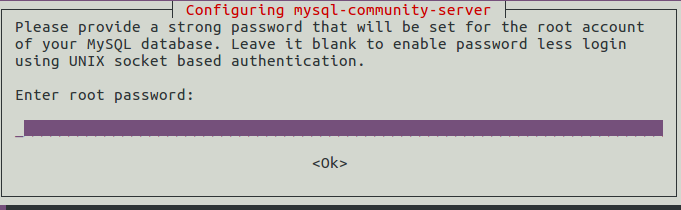
\includegraphics[scale=0.5]{formPasswordMySQLCommunityServer}
	}	\caption{Formulario de registro de contraseña para super usuario}
\end{figure}

De igual forma, volver a ingresar la anterior contraseña y presionar el botón 
\textquotedouble{Ok}.

\begin{figure}[!ht]
\centering
	\fbox{
		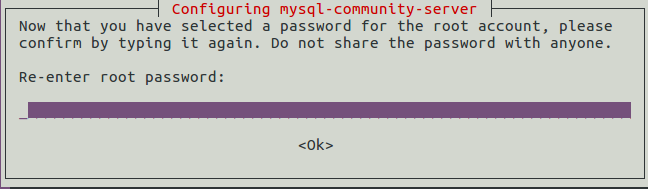
\includegraphics[scale=0.5]{formConfirmPasswordMySQLCommunityServer}
	}	\caption{Formulario de registro de contraseña para super usuario}
\end{figure}

A continuación, se instalar la librería dependencia del sistema operativo.

\begin{lstlisting}[language=bash, caption={Comando para instalar librería}]
# dpkg -i libaio1_0.3.110-2_amd64.deb 
\end{lstlisting}

Dicho lo anterior se ejecuta el comando, el cual integra la instalación de
forma resumida.

\begin{lstlisting}[language=bash, caption={Comando resumido de instalación de servidor de base de datos}]
# dpkg -i mysql-community-server_5.7.15-1ubuntu16.04_amd64.deb libmecab2_0996-1.2ubuntu1_amd64.deb
\end{lstlisting}

Igualmente, ejecutar el comando de instalacion de un cliente para el servidor
de base de datos.

\begin{lstlisting}[language=bash, caption={Comando de instalación de un cliente para el servidor}]
# dpkg -i mysql-community-client_5.7.15-1ubuntu16.04_amd64.deb 
\end{lstlisting}

Finalmente, ejecutar el comando de instalación de un cliente.

\begin{lstlisting}[language=bash, caption={Comando de instalacion de un cliente para el servidor}]
# dpkg -i libmysqlclient20_5.7.15-1ubuntu16.04_amd64.deb
\end{lstlisting}

\subsection{Apache2}

Si tu no tienes obtienes \textquotedouble{build-essential} paquete, instalar.

\begin{lstlisting}[language=bash, caption={Comandos para instalación de paquetes de compilación}]
# apt-get update
# apt-get install build-essential
\end{lstlisting}

Zlib una librería para comprimir métodos el cual se encontrado en gzip.

\begin{lstlisting}[language=bash, caption={Instalación dependencias para servidor web}]
# cd /usr/local/src
# tar xvfz zlib-1.2.8.tar.gz
# cd zlib-1.2.8/
# ./configure --prefix=/usr/local
# make
# make install
\end{lstlisting}

Actualmente se necesita instalar apr, por lo tanto realiza el siguiente
comando.

\begin{lstlisting}[language=bash, caption={Instalacion dependencias para servidor web}]
# cd /usr/local/src
# tar xvf apr-1.5.2.tar.gz
# cd apr-1.5.2
# ./configure
# make
# make install
\end{lstlisting}

Igualmente, utilizar la instalación de dependencia apr-util, utilitario del
servidor web.

\begin{lstlisting}[language=bash, caption={Instalación dependencias utilitarios para servidor web}]
# cd /usr/local/src
# tar xvf apr-util-1.5.4.tar.gz
# cd apr-util-1.5.4
# ./configure --with-apr=/usr/local/src/apr-1.5.2
# make
# make install
\end{lstlisting}

A continuación, se muestra como se debe instalar otra dependencia del servidor
web.

\begin{lstlisting}[language=bash, caption={Instalación de otra dependencia del servidor web}]
# apt-get update
# apt-get install libpcre3-dev
\end{lstlisting}

Por lo tanto, utilizar los comandos para realizar la instalación del servidor web.

\begin{lstlisting}[language=bash, caption={Instalación de un servidor web}]
# cd /usr/local/src
# tar xvf http-2-4.23.tar.gz
# cd http-2.4.23
# ./configure --prefix=/usr/local/apache --enable-so 
# make
# make install
\end{lstlisting}

Realizar una copia y brindar permisos de ejecución.

\begin{lstlisting}[language=bash, caption={Comandos para agregar como demonio}]
# cp /usr/local/apache/bin/apachectl /etc/init.d/apachectl
# chmod +x /etc/init.d/apachectl
\end{lstlisting}

\textbf{actualizar-rc}

\begin{lstlisting}[language=bash, caption={}]
# /usr/sbin/update-rc.d -f apachectl defaults
\end{lstlisting}

Seguridad apache

\begin{lstlisting}[language=bash, caption={}]
# adduser --system apache
\end{lstlisting}

ahora, nosotros necesitamos hacer seguro apache ejecute este usuario.

\begin{lstlisting}[language=bash, caption={}]
# nano /usr/local/apache/conf/httpd.conf
\end{lstlisting}

tu necesitas find estas lineas:

\begin{lstlisting}[language=bash, caption={}]
User daemon
Group daemon
\end{lstlisting}

y ahora cambiar por lo siguiente.

\begin{lstlisting}[language=bash, caption={}]
User apache
Group nogroup
\end{lstlisting}

guardar el archivo, restaurar el servicio.

\begin{lstlisting}[language=bash, caption={}]
# /usr/local/apache/bin/apachectl start
\end{lstlisting}

como se afirmo arriba, se procede a realizar la verificación de la instalación
por uso de un navegador web, para luego escribir \textquotedouble{http://localhost}. 

\begin{figure}[!ht]
\centering
	\fbox{
		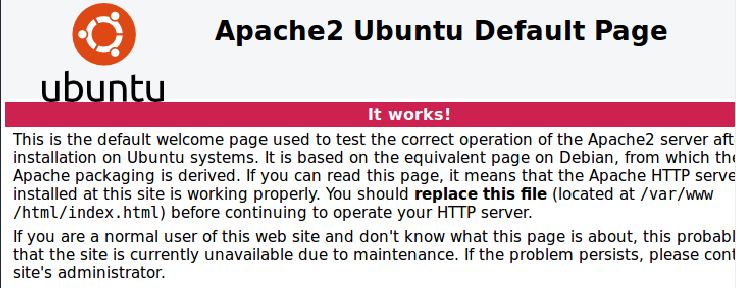
\includegraphics[scale=0.5]{verifyApacheBrowser}
	}	\caption{Verificación ejecución página por defecto de apache}
\end{figure}


\subsection{PHP}

Por lo que se refiere a, lenguaje lado del servidor.

\begin{lstlisting}[language=bash, caption={Comando para instalación de lenguaje en el lado del servidor}]
# apt-get update
# apt-get install php7.0-mysql php7.0-curl php7.0-curl php7.0-cgi php7.0 libapache2-mod-php7
# /usr/local/apache/bin/apachectl stop
# /usr/local/apache/bin/apachectl start
\end{lstlisting}

\subsection{Configuración}

A continuación, se define la ruta a utilizar para el proceso de instalación de
la aplicación \textquotedouble{/media/TrabajoDeGrado/Fuentes}

\subsection{Plataforma educativa LAEL}

\begin{itemize}

\item \textbf{Aplicación web}

Para poder hacer acceso de la aplicación se utilizara la ruta 
\textquotedouble{/media/TrabajoDeGrado/Fuentes/Código}

A continuación, realizar con la instalación de la aplicación.

\begin{lstlisting}[language=bash, caption={}]
# cp /media/TrabajoDeGrado/Fuentes/plafromaeducativalael.zip /usr/local/apache/htdocs/
# cd /usr/local/apache/htdocs/
# unzip plataformaeducativalael.zip
# chmod -R 7555 ./plataformaeducativalael
# cd plataformaeducativalael
# mkdir assets
\end{lstlisting}

\item \textbf{Base de datos}

Para poder hacer acceso de la aplicación se utilizara la ruta 
\textquotedouble{/media/TrabajoDeGrado/Fuentes/Bd}

\begin{lstlisting}[language=bash, caption={}]
# cp /media/TrabajoDeGrado/Bd/BDplafromaeducativalael.zip /home/ubuntu
# cd /home/ubuntu
# unzip BDplataformaeducativalael.zip
# mysql --host=localhost --user=root
> create database plataformaeducativalael;
> exit;
# mysql --host=localhost --user=root plataformaeducativalael < BDplataformaeducativalael.sql
\end{lstlisting}
\end{itemize}
